For modeling QoE, there have been numerous studies that take into account video content-related factors (e.g., type of video, the complexity of video, etc.). However, most of them neglected the user's interest, in other words, DoI. In fact, influenced by video content and viewer preferences, the user possibly has different DoI on different videos or different parts of a video. Intuitively, the user seems to provide higher QoE scores for the video with interesting content and vice versa. Typically, Degree-of-Interest (DoI) \cite{DegreeOfLiking_SOS} is defined as the interestingness of the video content, or the ability of the video content to attract the user and keep the user's interest \cite{VisualContent}.

To make this clear, we investigate the correlation between DoI and the overall QoE by conducting a subjective test. In this test, 18 undistorted videos from the LFOVIA Database \cite{LFOVIA} were utilized. The video content varied upon nature, wildlife, outdoor, marine, sports, animation, and gaming \cite{LFOVIA} among every video, each of which the duration is 120 seconds. This guaranteed that the subjects would retain their interests as they watched.
%The snapshots of these videos are shown in Figure \ref{fig:snapshots}.
The referenced videos were randomly divided into 6 collections and encoded using FFmpeg \cite{FFmpeg} under the default settings with the resolution of 1920 x 1080 and were displayed on a 15-inch monitor with a resolution of 1920 x 1080 and a black background. The Absolute Category Rating (ACR) \cite{ITUT_P913} method was used and there were 60 subjects agreed to participate in this experiment. Each video was assessed by at least 10 subjects. At the end of each video, the subject was asked to give an overall score representing his/her interest in the entire video content, ranging from 1 (worst or not at all interested) to 5 (best or extremely interested), following the general principle of the ITU-T recommendation P.913 \cite{ITUT_P913}. A 3-minute break was provided to each subject between each video to minimize the effects of viewer fatigue. The average of subjects' scores or Mean Opinion Score (MOS) for each video was utilized as the DoI of video. These values were then linearly scaled up to the range of 0 to 100 and compared with the corresponding overall QoE in the LFOVIA Database.

\begin{figure}[tb]
  \begin{center}
    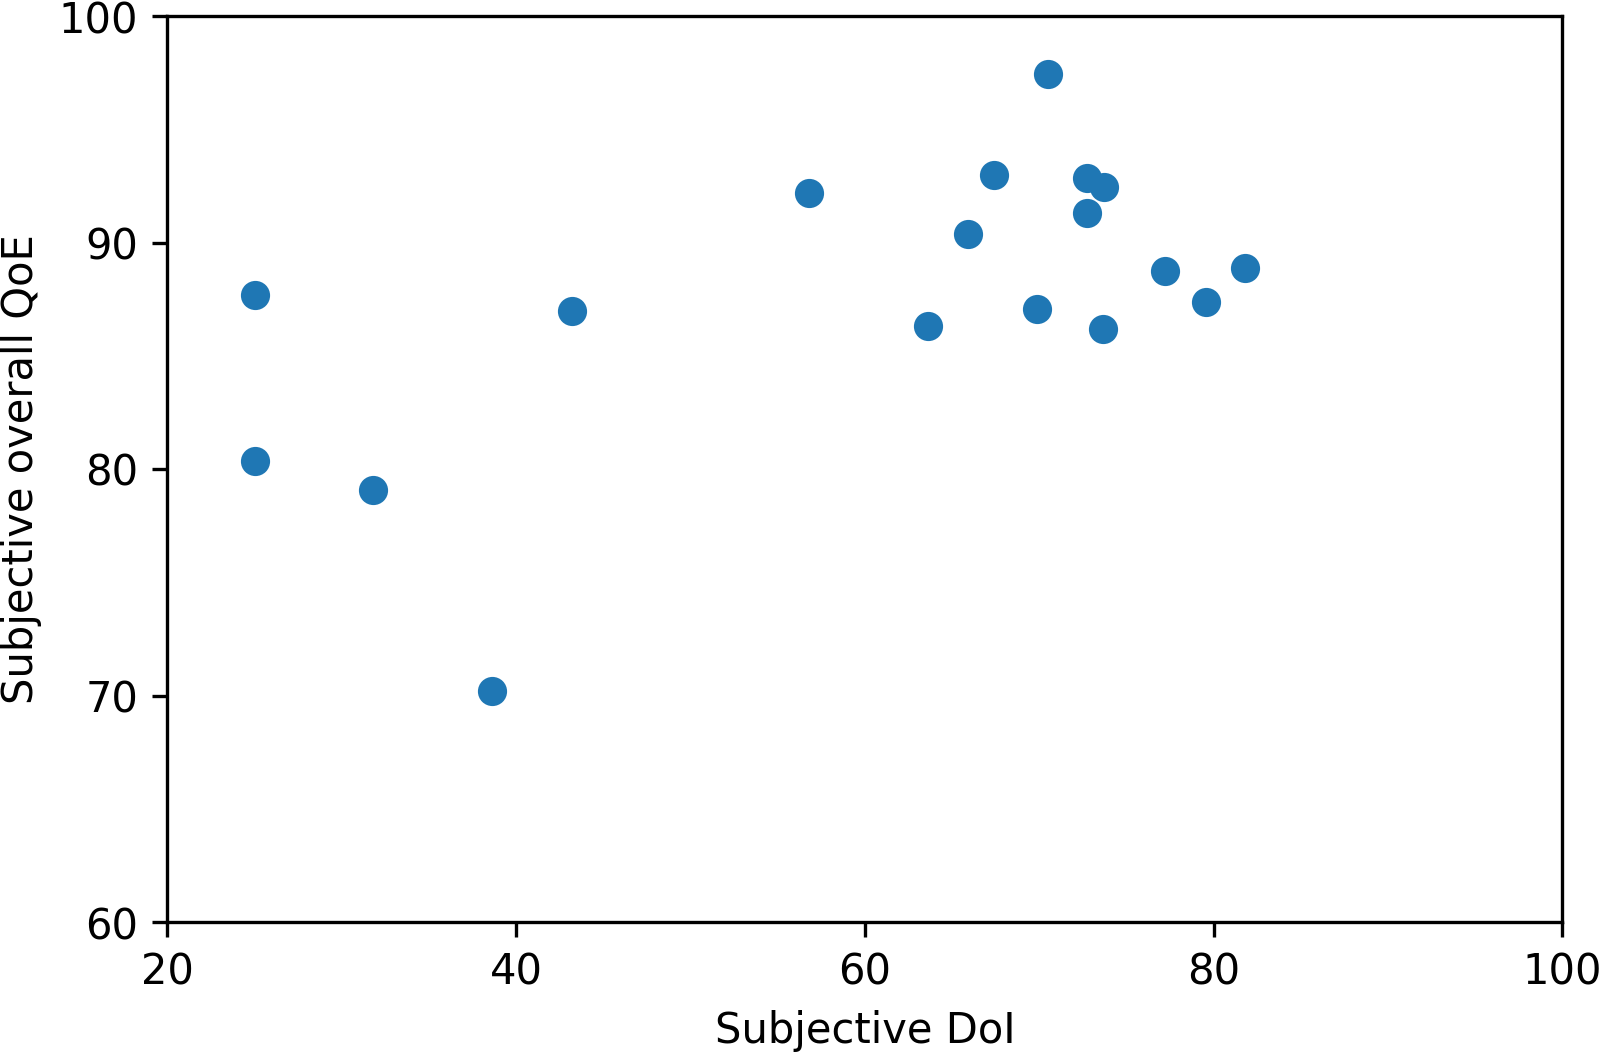
\includegraphics[width=0.6\linewidth]{\FigsDir/pcc_doi_overallqoe.png}
  \end{center}
  \caption{Scatter plot between the mean of subjective DoI scores and the subjective overall QoE obtained in the database.}
  \label{fig:PCC_DoI_OverallQoE}
\end{figure}

Figure \ref{fig:PCC_DoI_OverallQoE} illustrates the obtained correlation between DoI and the overall QoE, which achieved the Pearson Correlation Coefficient (PCC) of \textbf{0.601}. The correlation was modest. We speculate this as the small number of subjects participating in the experiment. Yet, it is shown that the DoI has an influence on the final decisions of the users when they provide the overall QoE. In the future, a larger number of subjects will be considered for further investigation. Based on the conclusion of this experiment, we introduce DoI as one of the potential influence factors in the proposed cumulative QoE model.
